\section{VertexCDA}

\newcommand{\p}[1]{\vec{p}_{#1}}
\newcommand{\ap}[1]{|\vec{p}_{#1}|^2}
\newcommand{\lv}{\vec{l}}
\newcommand{\lz}{\vec{l}_{0}}
\newcommand{\C}[1]{\vec{A}_{#1}}
\newcommand{\x}[1]{\vec{x}_{#1}}

The aim of this analyzer is to implement an algorithm that will compute the Kaon
decay vertex and make it available to further analyzers. Though different
methods are available for this purpose, the focus is given on a closest distance
of approach (CDA) algorithm. The algorithm implemented by this analyzer can be
used for the class of processes $K^\pm\to C^\pm X$ where $K^\pm$ is the
incoming charged Kaon measured in GigaTracker, $C^\pm$ is a charged particle
measured in the Spectrometer and $X$ is any kind and any number of additional particle. Even if the
tracks are supposed to originate from the same point they are in practice never intersecting
because of the finite measurement precision. As long as the tracks are not parallel the CDA will
find the unique point $\vec{V}=(V_x,V_y,V_z)$ where the distance between $\vec{V}$ and the first
track and the distance between $\vec{V}$ and the second track are minimums. For this point only,
the vector $\lv$ passing through $\vec{V}$ and joining both tracks is perpendicular to
them.

If the track origins $\vec{x}_{1,2}$ and their momenta $\p{1,2}$ are defined, any point $\C{1,2}$
on track can be described by the parameter $s_{1,2}$ such as
\begin{equation}
	\C{1,2} = \x{1,2} + s_{1,2} \p{1,2}
\end{equation}

The vector joining $\C{1}$ and $\C{2}$ is then
\begin{eqnarray}
	\lv(s_1,s_2)=\C{1}-\C{2} &=& \x{1}+s_1\p{1} - \x{2} - s_2\p{2}\\
%	&=& \x{1}-\x{2} + s_1\p{1} - s_2\p{2}\\
	&=& \lz + s_1\p{1} - s_2\p{2}
\end{eqnarray}
with $\lz = \x{1}-\x{2}$. Using the property that $\lv$ is perpendicular to
$\p{1}$ and $\p{2}$ when its length is minimum gives the following
equations:

\begin{align}
	\lv(s_{1c},s_{2c})\cdot\p{1} &= \lz\cdot\p{1} + s_{1c}\ap{1} -
	s_{2c}(\p{1}\cdot\p{2}) &= 0
	\\
	\lv(s_{1c},s_{2c})\cdot\p{2} &= \lz\cdot\p{2} + s_{1c}(\p{2}\cdot\p{1}) -
	s_{2c}\ap{2} &= 0
\end{align}
They can be solved for $s_{1c}$ and $s_{2c}$:

\begin{align}
	s_{1c} &= \frac{(\p{1}\cdot\p{2})(\lz\cdot\p{2}) -
	(\lz\cdot\p{1})\ap{2}}{\ap{1}\ap{2} - (\p{1}\cdot\p{2})^2}\\
	s_{2c} &= \frac{\ap{1}(\lz\cdot\p{2}) -
	(\p{1}\cdot\p{2})(\lz\cdot\p{1})}{\ap{1}\ap{2} - (\p{1}\cdot\p{2})^2}
\end{align}

The vertex being in the middle of the $\lv(s_{1c},s_{2c})$ vector:
\begin{equation}
	\vec{V} = \C{1} + 0.5\lv(s_{1c},s_{2c})
\end{equation}

\subsection{VertexCDA analyzer implementation}
The first step is to create the skeleton of the new analyzer. This is
automatically done with the framework python script:
\begin{lstlisting}
NA62AnalysisBuilder.py new VertexCDA
\end{lstlisting}

The source code of the newly created analyzer can be found in
\path{Analyzers/include/VertexCDA.hh} and \path{Analyzers/src/VertexCDA.cc}. Every standard method
of the analyzer and each section of code will be described thereafter.

\subsubsection{Constructor}
As the GigaTracker and Spectrometer information needs to be accessed, it is necessary to start by 
requesting these ROOT TTrees:

\begin{lstlisting}
//Request TTree with name GigaTracker with elements of class TRecoGigaTrackerEvent
RequestTree("GigaTracker", new TRecoGigaTrackerEvent);
//Request TTree with name Spectrometer with elements of class TRecoSpectrometerEvent
RequestTree("Spectrometer", new TRecoSpectrometerEvent);
\end{lstlisting}
 
 Without forgetting to include the relevant header files at the beginning of the file
\begin{lstlisting}
#include "TRecoGigaTrackerEvent.hh"
#include "TRecoSpectrometerEvent.hh"
\end{lstlisting}

\subsubsection{InitHist}
In this method all the histograms that will be needed during the processing are created and
registered to the framework:

\begin{itemize}
  \item Histograms for plotting the vertex x,y,z positions
\begin{lstlisting}
//Booking 3 histograms to plot the reconstructed vertex x,y,z positions
//Book Histogram VertexX (name that will be used to access this histogram later) and 
//create it with new TH1I (see ROOT TH1I for the syntax).
BookHisto("VertexX", 
	new TH1I("VertexX", "Reconstructed vertex X position", 250, -250, 250));
BookHisto("VertexY", 
	new TH1I("VertexY", "Reconstructed vertex Y position", 150, -150, 150));
BookHisto("VertexZ", 
	new TH1I("VertexZ", "Reconstructed vertex Z position", 100, 0, 300000));
\end{lstlisting}
	\item Histograms to compare the reconstructed vertex with the true Monte Carlo vertex
\begin{lstlisting}
//Booking 3 histograms to plot the difference between the reconstructed vertex and the real vertex components
BookHisto("DiffVertexX", 
	new TH1I("DiffVertexX", "X difference between reco and real vertex", 200, -50, 50));
BookHisto("DiffVertexY", 
	new TH1I("DiffVertexY", "Y difference between reco and real vertex", 200, -50, 50));
BookHisto("DiffVertexZ", 
	new TH1I("DiffVertexZ", "Z difference between reco and real vertex", 200, -10000, 10000));

//Booking 3 2D histograms to plot the reconstructed vertex components vs. the real vertex components
BookHisto("VertexRecoRealX", 
	new TH2I("VertexRecoRealX", "Reconstructed vs. Real (X)", 250, -250, 250, 250, -250, 250));
BookHisto("VertexRecoRealY", 
	new TH2I("VertexRecoRealY", "Reconstructed vs. Real (Y)", 150, -150, 150, 150, -150, 150));
BookHisto("VertexRecoRealZ", 
	new TH2I("VertexRecoRealZ", "Reconstructed vs. Real (Z)", 200, 0, 300000, 200, 0, 300000));
\end{lstlisting}
	\item Histograms for the particle multiplicity in detectors
\begin{lstlisting}
//Booking histograms to plot the reconstructed candidates multiplicity in GigaTracker and Spectrometer
BookHisto("GTKMultiplicity", 
	new TH1I("GTKMultiplicity", "Multiplicity in GTK", 11, -0.5, 10.5));
BookHisto("StrawMultiplicity", 
	new TH1I("StrawMultiplicity", "Multiplicity in Straw", 11, -0.5, 10.5));
\end{lstlisting}
	\item A serie of histogram to plot the kaon decay profile in 20 z sections
\begin{lstlisting}
//Booking a serie of 20 histogram to plot the MC Kaon decay vertex X-Y profile in different sections
of the detector length 
for(int i=0; i<20; i++){
	BookHisto(TString("BeamXY") + (Long_t)i, 
		new TH2I(TString("BeamXY") + (Long_t)i,
				TString("BeamXY") + (Long_t)(100+i*5) + TString("->") + (Long_t)(100+(i+1)*5),
				100, -100, 100, 100, -100, 100));
}
\end{lstlisting}
\end{itemize}

Several counters to keep track of the number of events passing the selection are created as well.
The counters are grouped in an \class{EventFraction} table and the sample size for this table is
defined as the \refcode{Total\_Events} counter.

\begin{lstlisting}
BookCounter("Total_Events");
BookCounter("Good_GTK_Mult");
BookCounter("Good_Straw_Mult");

NewEventFraction("Selection");
AddCounterToEventFraction("Selection", "Total_Events");
AddCounterToEventFraction("Selection", "Good_GTK_Mult");
AddCounterToEventFraction("Selection", "Good_Straw_Mult");
DefineSampleSizeCounter("Selection", "Total_Events");
\end{lstlisting} 

\subsubsection{InitOutput}
This analyzer is meant to provide a vertex to other analyzers. The \var{fVertex} member object is
first declared in the header of the analyzer:

\begin{lstlisting}
protected:
	TVector3 fVertex;
\end{lstlisting}
Before declaring it to the framework under the name \refcode{Vertex} in the \method{InitOutput}
method. It should be noted that to avoid collisions between independent analyzers, this name is
automatically prepended with the name of the analyzer and a dot. In this case, to access this
object from another analyzer, one will have to request \refcode{VertexCDA.Vertex}

\begin{lstlisting}
RegisterOutput("Vertex", &fVertex);
\end{lstlisting}

\subsubsection{DefineMCSimple}
This method is specific to simulated events. A specific partial event signature of the type
$K^+\to\pi^+X$ is defined where $X$ can be any number (0 included) of any particle. When reading
simulated events, the list of simulated particles (\class{KineParts}) will be scanned and the
particles corresponding to the definition given here will be stored in a structure that will allow
to easily referencing them later.

\begin{lstlisting}
//We ask for the initial Kaon and store it's ID
int kID = fMCSimple->AddParticle(0, 321);
// We ask for the positive pion whose parent is the initial Kaon (kID as parent)
fMCSimple->AddParticle(kID, 211);
\end{lstlisting}

\subsubsection{Process}
This method is the main process loop. Every event will be processed by this method. First some
variable declaration:
\begin{lstlisting}
//Flags for rejected/accepted events
bool badEvent = false;
//Will contain the Kaon position on GigaTracker station 3 and it's reconstructed momentum
TVector3 KaonPosition, KaonMomentum;
//Will contain the charged pion position returned by Spectrometer and it's reconstructed momentum 
TVector3 PipPosition, PipMomentum;
\end{lstlisting}

This analyzer does not need simulated data but can do extra-work for consistency checks if
available. The use of simulated data is therefore not enforced but it is checked anyway and the
\var{withMC} flag is set accordingly. The \var{fMCSimpe.fStatus} flag can take 3 different values:
\begin{itemize}
  \item \var{kEmpty}: No Monte Carlo data have been found
  \item \var{kMissing}: Monte Carlo data have been found but the current event does not correspond
  to the signature given in \method{DefineMCSimple} 
  \item \var{kComplete}: Monte Carlo data have been found and the event corresponds to the signature
  given in \method{DefineMCSimple}. There could be additional particles in the event.
\end{itemize}
The extra-work can only be realized with a complete event and therefore only events with the value
\var{KComplete} are relevant.

\begin{lstlisting}
//Declare the flag
bool withMC = true;
//For the additional jobWe are only interested in complete 
if(fMCSimple.fStatus != MCSimple::kComplete) withMC = false;
\end{lstlisting}

Then the events retrieved from the GigaTracker and Spectrometer TTrees are retrieved
\begin{lstlisting}
TRecoGigaTrackerEvent *GTKEvent = (TRecoGigaTrackerEvent*)GetEvent("GigaTracker");
TRecoSpectrometerEvent *SpectrometerEvent = (TRecoSpectrometerEvent*)GetEvent("Spectrometer");
\end{lstlisting}

And the counter that keeps track of the total number of processed events is incremented
\begin{lstlisting}
IncrementCounter("Total_Events");
\end{lstlisting}

The next step is handling the GigaTracker information. The multiplicity histogram are filled,
and the Kaon variables are set only if 1 candidate has been reconstructed. The Kaon position is the
position on station 3 but as the coordinates are relative to the centre of the GigaTracker
detector, it has to be translated into the experiment frame. Only the z coordinate is impacted.
The counter keeping the count of events passing the GigaTracker selection is incremented as well.
The event is flagged as bad if 0 or more than 1 candidates are reconstructed.

\begin{lstlisting}
//Filling GigaTracker multiplicity histogram
FillHisto("GTKMultiplicity", GTKEvent->GetNCandidates());
if(GTKEvent->GetNCandidates()==1){
	//If only 1 reconstructed candidate, set KaonPosition to the position on station 3 (index 2)
	KaonPosition = ((TRecoGigaTrackerCandidate*)GTKEvent->GetCandidate(0))->GetPosition(2);
	//Move Z to the experiment frame. Z position of GigaTracker centre is 90932.5mm  
	KaonPosition.SetZ(KaonPosition.Z()+90932.5);
	//Set the Kaon momentum as measured by GigaTracker
	KaonMomentum = ((TRecoGigaTrackerCandidate*)GTKEvent->GetCandidate(0))->GetMomentum().Vect();
	//Increment the GigaTracker selection counter
	IncrementCounter("Good_GTK_Mult");
}
else badEvent = true;
\end{lstlisting}

The same processing is applied for the reconstructed Spectrometer events. The multiplicity 
histogram is filled then the position and momentum are set if only one candidate is reconstructed
and the counter for the Spectrometer selection is incremented. If no or more than one event is
found, the \var{badEvent} flag is raised.

\begin{lstlisting}
FillHisto("StrawMultiplicity", SpectrometerEvent->GetNCandidates());
if(SpectrometerEvent->GetNCandidates()==1){
	PipPosition = ((TRecoSpectrometerCandidate*)SpectrometerEvent->GetCandidate(0))->GetPosition();
	PipMomentum = ((TRecoSpectrometerCandidate*)SpectrometerEvent->GetCandidate(0))->GetMomentum().Vect();
	IncrementCounter("Good_Straw_Mult");
}
else badEvent = true;
\end{lstlisting}

Finally if the event is tagged as bad, the state of the output is set to \var{kOInvalid} without
further treatment to signal other analyzers that the value of this output should not be used. 

\begin{lstlisting}
if(badEvent){
	//Signal the state of the Vertex output as kOInvalid if the event did not pass the selection
	SetOutputState("Vertex", kOInvalid);
}
\end{lstlisting}

If the event passed the selection, the vertex is finally computed with the CDA algorithm (whose
implementation is described in section \ref{GetIntersection}), the state of the output is set to
\var{kOValid} to signal other analyzers that they can use it, and the three Vertex histograms are
filled.

\begin{lstlisting}
else{
	//Get the vertex from the CDA algorithm
	fVertex = GetIntersection(KaonPosition, KaonMomentum, PipPosition, PipMomentum);
	\\Signal the state of the Vertex Output as kOValid
	SetOutputState("Vertex", kOValid);
	
	//Fill the histograms with the vertex components
	FillHisto("VertexX", fVertex.X());
	FillHisto("VertexY", fVertex.Y());
	FillHisto("VertexZ", fVertex.Z());
\end{lstlisting}

To finish the event processing, and if Monte Carlo are available, the reconstructed vertex is
compared to the real one component by component and the results are inserted in 1D and 2D
histograms. The vertex X-Y profile along the experiment is also plotted in 20 z sections starting
at z=100m.
\begin{lstlisting}
	if(withMC){
		FillHisto("DiffVertexX", fVertex.X()-fMCSimple["pi+"][0]->GetProdPos().X());
		FillHisto("DiffVertexY", fVertex.Y()-fMCSimple["pi+"][0]->GetProdPos().Y());
		FillHisto("DiffVertexZ", fVertex.Z()-fMCSimple["pi+"][0]->GetProdPos().Z());
		FillHisto("VertexRecoRealX", fVertex.X(), fMCSimple["pi+"][0]->GetProdPos().X());
		FillHisto("VertexRecoRealY", fVertex.Y(), fMCSimple["pi+"][0]->GetProdPos().Y());
		FillHisto("VertexRecoRealZ", fVertex.Z(), fMCSimple["pi+"][0]->GetProdPos().Z());
		int cat = ((fMCSimple["pi+"][0]->GetProdPos().Z()/1000)-100)/5;
		FillHisto(TString("BeamXY") + (Long_t)cat, fMCSimple["pi+"][0]->GetProdPos().X(), fMCSimple["pi+"][0]->GetProdPos().Y());
	}
}
\end{lstlisting}

\subsubsection{PostProcess}
This method is meant to destroy temporary objects that have been allocated during \method{Process}
and that shall be destroyed only after all the analyzers finished processing the event. This is
typically the case for memory allocated for the output of the analyzer. In the specific case of this
analyzer, no such memory has been allocated and this method will stay empty.

\subsubsection{ExportPlot}
All the histograms previously booked with \method{BookHisto} are saved in the output ROOT file with

\begin{lstlisting}
SaveAllPlots();
\end{lstlisting} 

\subsubsection{DrawPlot}
Similarly if the analysis is running in graphical mode, all the histograms previously booked with
\method{BookHisto} should be displayed on screen:

\begin{lstlisting}
DrawAllPlots();
\end{lstlisting} 

\subsubsection{GetIntersection}\label{GetIntersection}
This is the implementation of the CDA algorithm described earlier in this document. As input it
receive two 3-vectors \var{x1} and \var{x2} being respectively a point belonging to the first track
and a point belonging to the second track, and two 3-vector \var{p1} and \var{p2} representing the
directions of the tracks.

The \var{l0} vector is determined from the positions: 
\begin{lstlisting}
TVector3 l0 = x1-x2;
\end{lstlisting}
Then the different cross-products and the $s_{1,2}$ parameters are computed:
\begin{lstlisting}
double a = p1.Mag2();
double b = p1*p2;
double c = p2.Mag2();
double d = p1*d0;
double e = p2*d0;
double s1 = (b*e-c*d)/(a*c-b*b);
double s2 = (a*e-b*d)/(a*c-b*b);
\end{lstlisting}
The vector linking the closest points ($\lv(s_1, s_2)$ in the algorithm) is \var{vdist} and the
point $\vec{V}$ being in the middle of this vector is returned:
\begin{lstlisting}
TVector3 vdist = l0 + (s1*p1 - s2*p2);

return x1 + s1*p1 - 0.5*vdist;
\end{lstlisting}

\subsection{Validation}
The figure \ref{vertexcdavalidation} shows one of the results  of the \class{VertexCDA} analyzer.
The two top histograms display the x and z values of the reconstructed vertex and the bottom ones
display a gaussian fit of the difference between the reconstructed and the real vertex x and z
values. The reconstructed x axis gaussian is centered around 0 with a very small standard deviation
of less than 1mm. The y axis is similar to x. The z axis is slightly displaced of $(7\pm1)$mm with a
variance of $(27.3\pm0.2)$cm. The tracks measured points being spaced of more than 100m and the
scale of the decay zone being of 65m the relative error is smaller than the $1\%$ level.
\begin{figure}
\begin{subfigure}{0.5\textwidth}
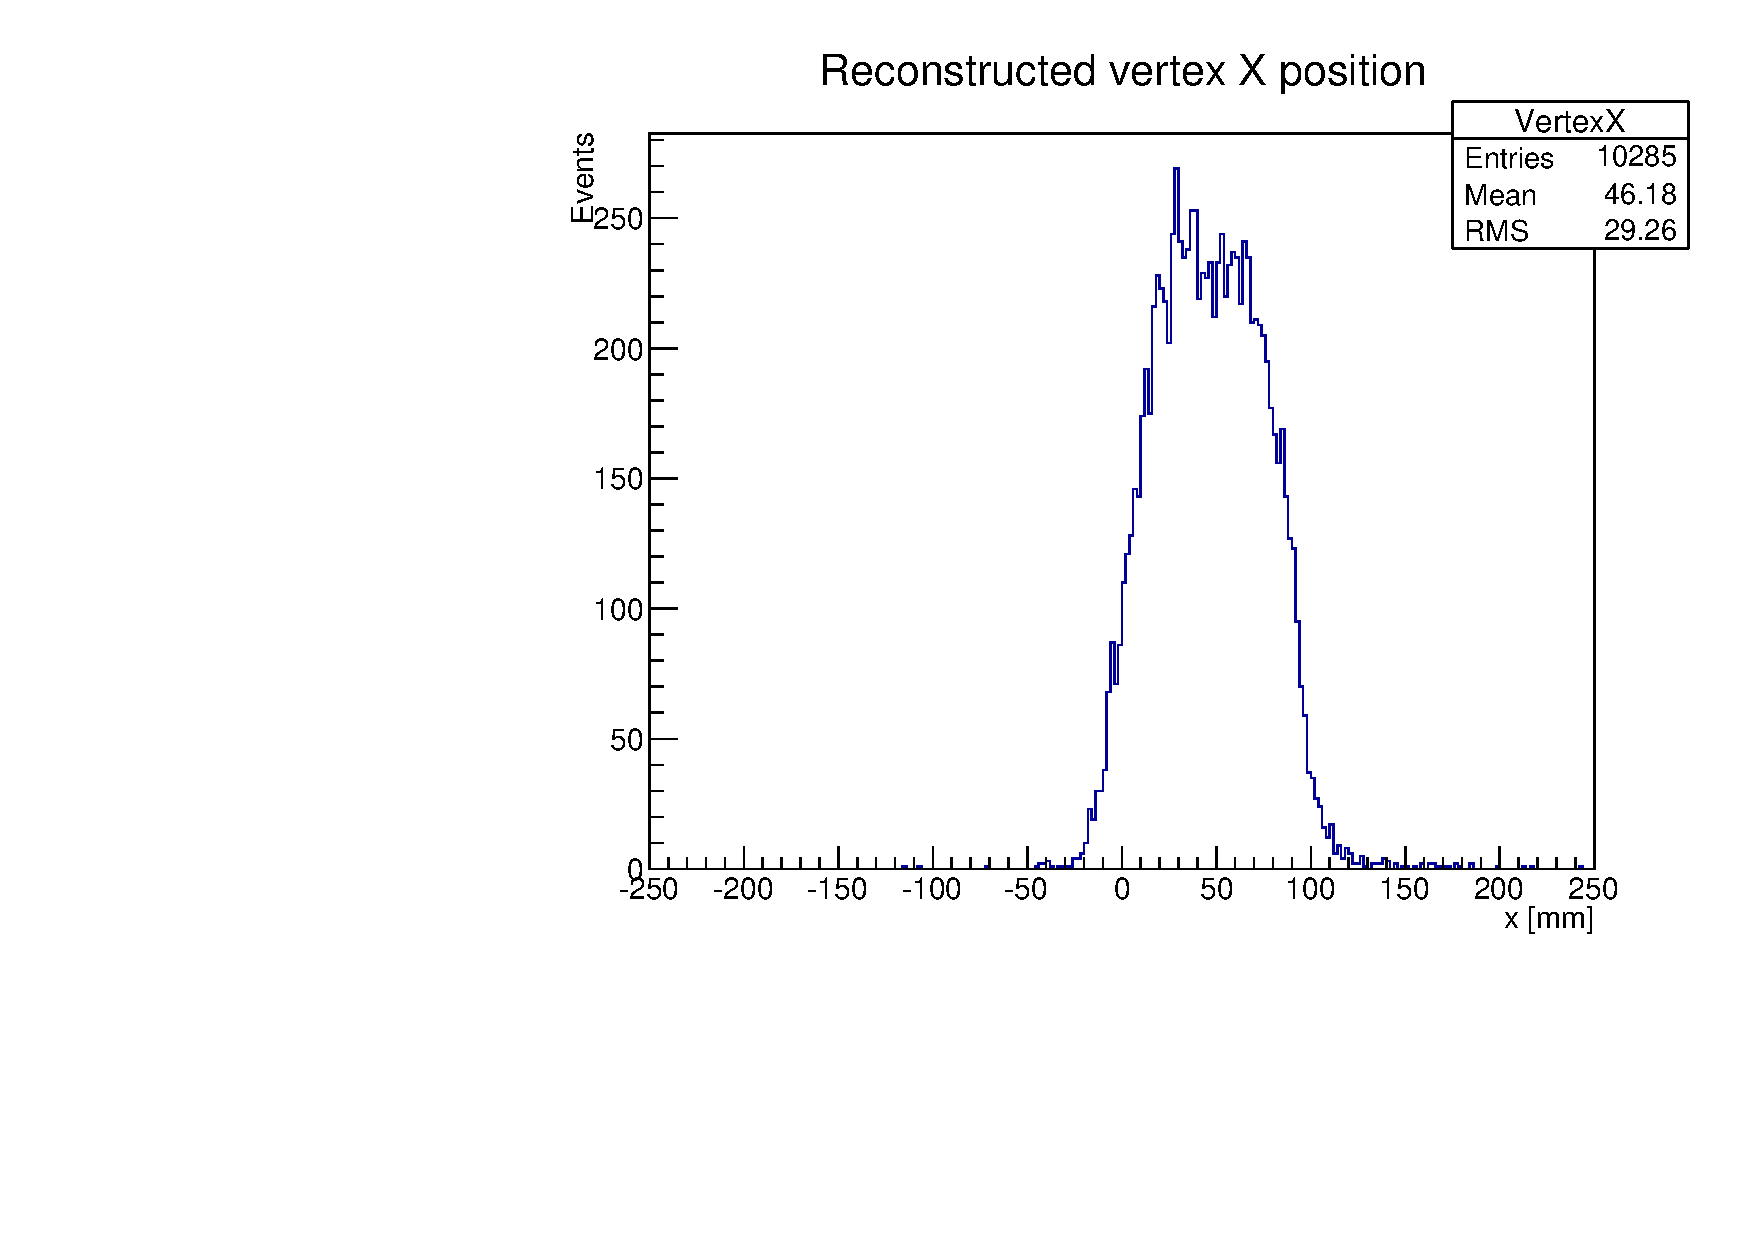
\includegraphics[width=\textwidth]{cdax}
\end{subfigure}
\begin{subfigure}{0.5\textwidth}
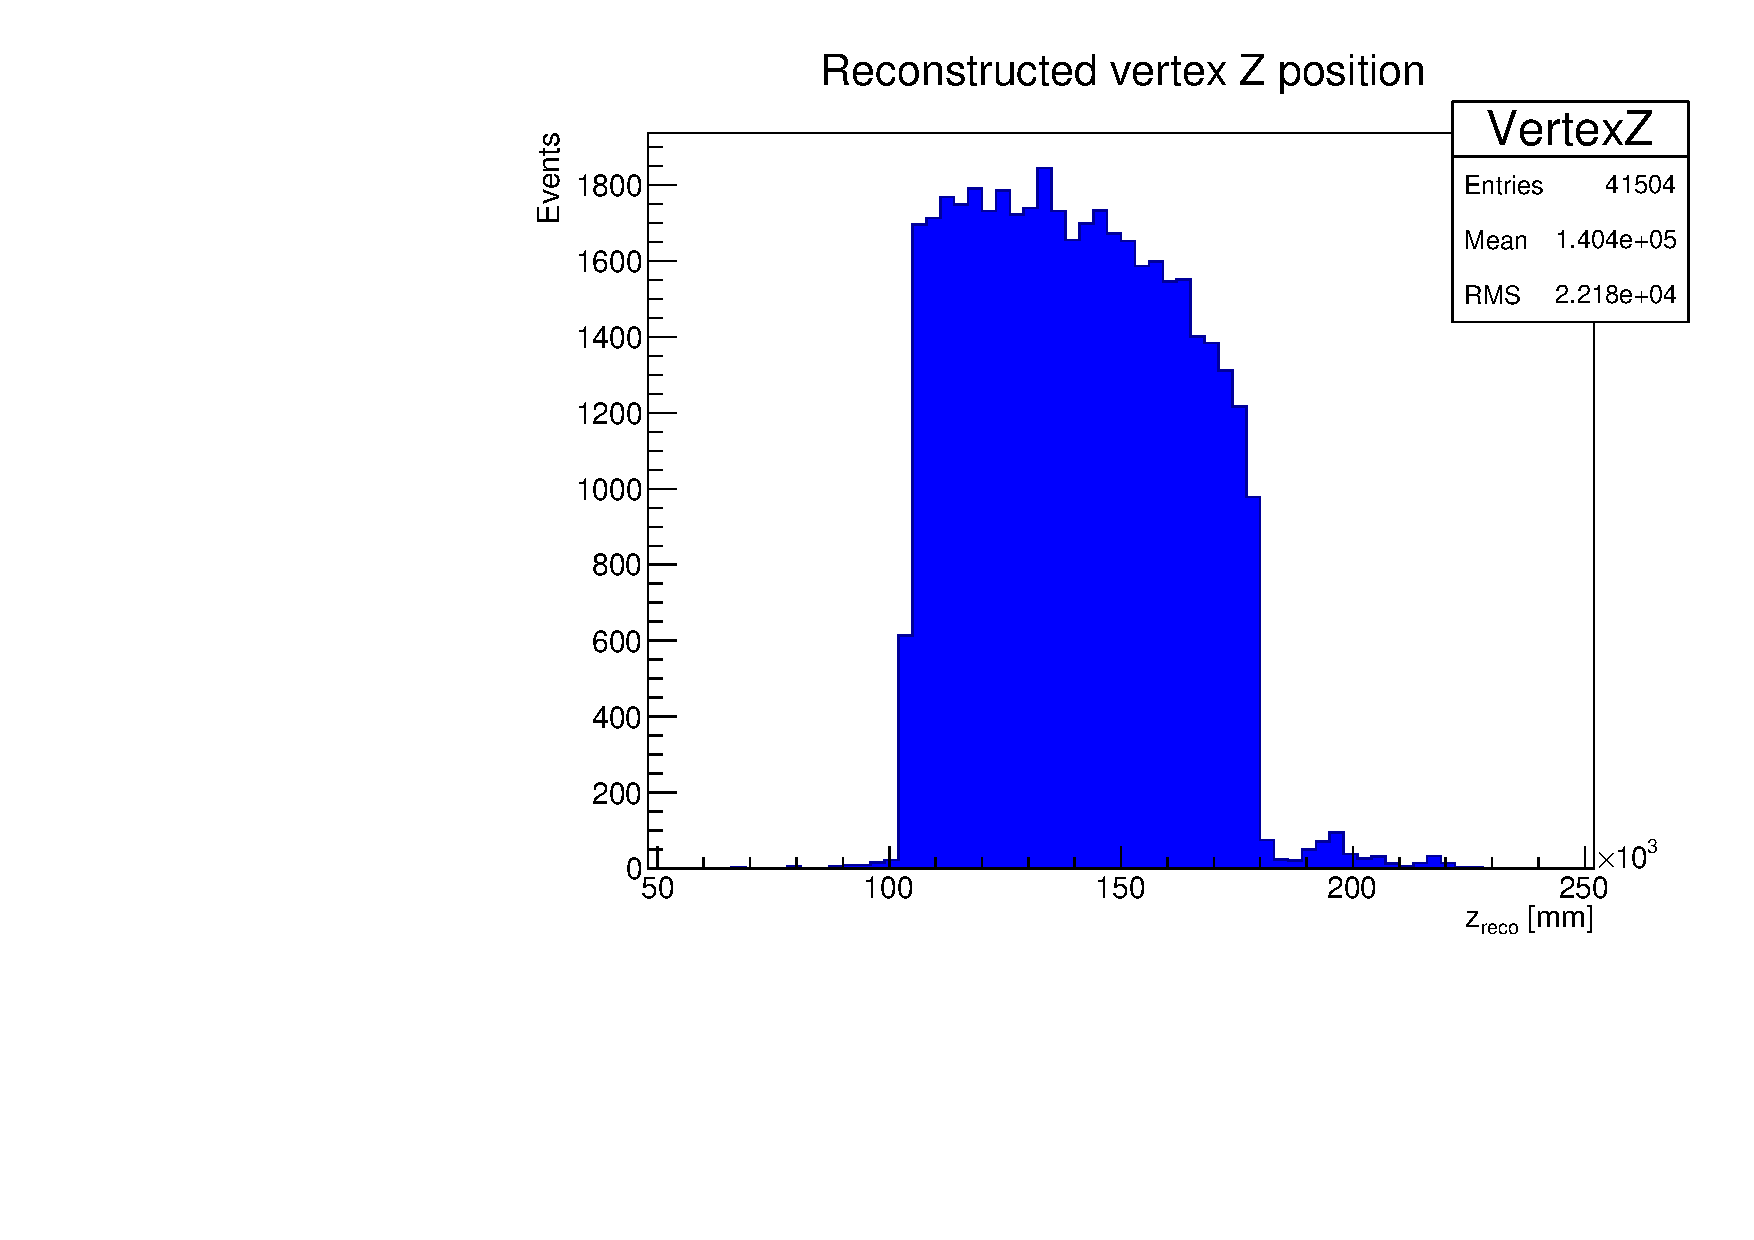
\includegraphics[width=\textwidth]{cdaz}
\end{subfigure}\\
\begin{subfigure}{0.5\textwidth}
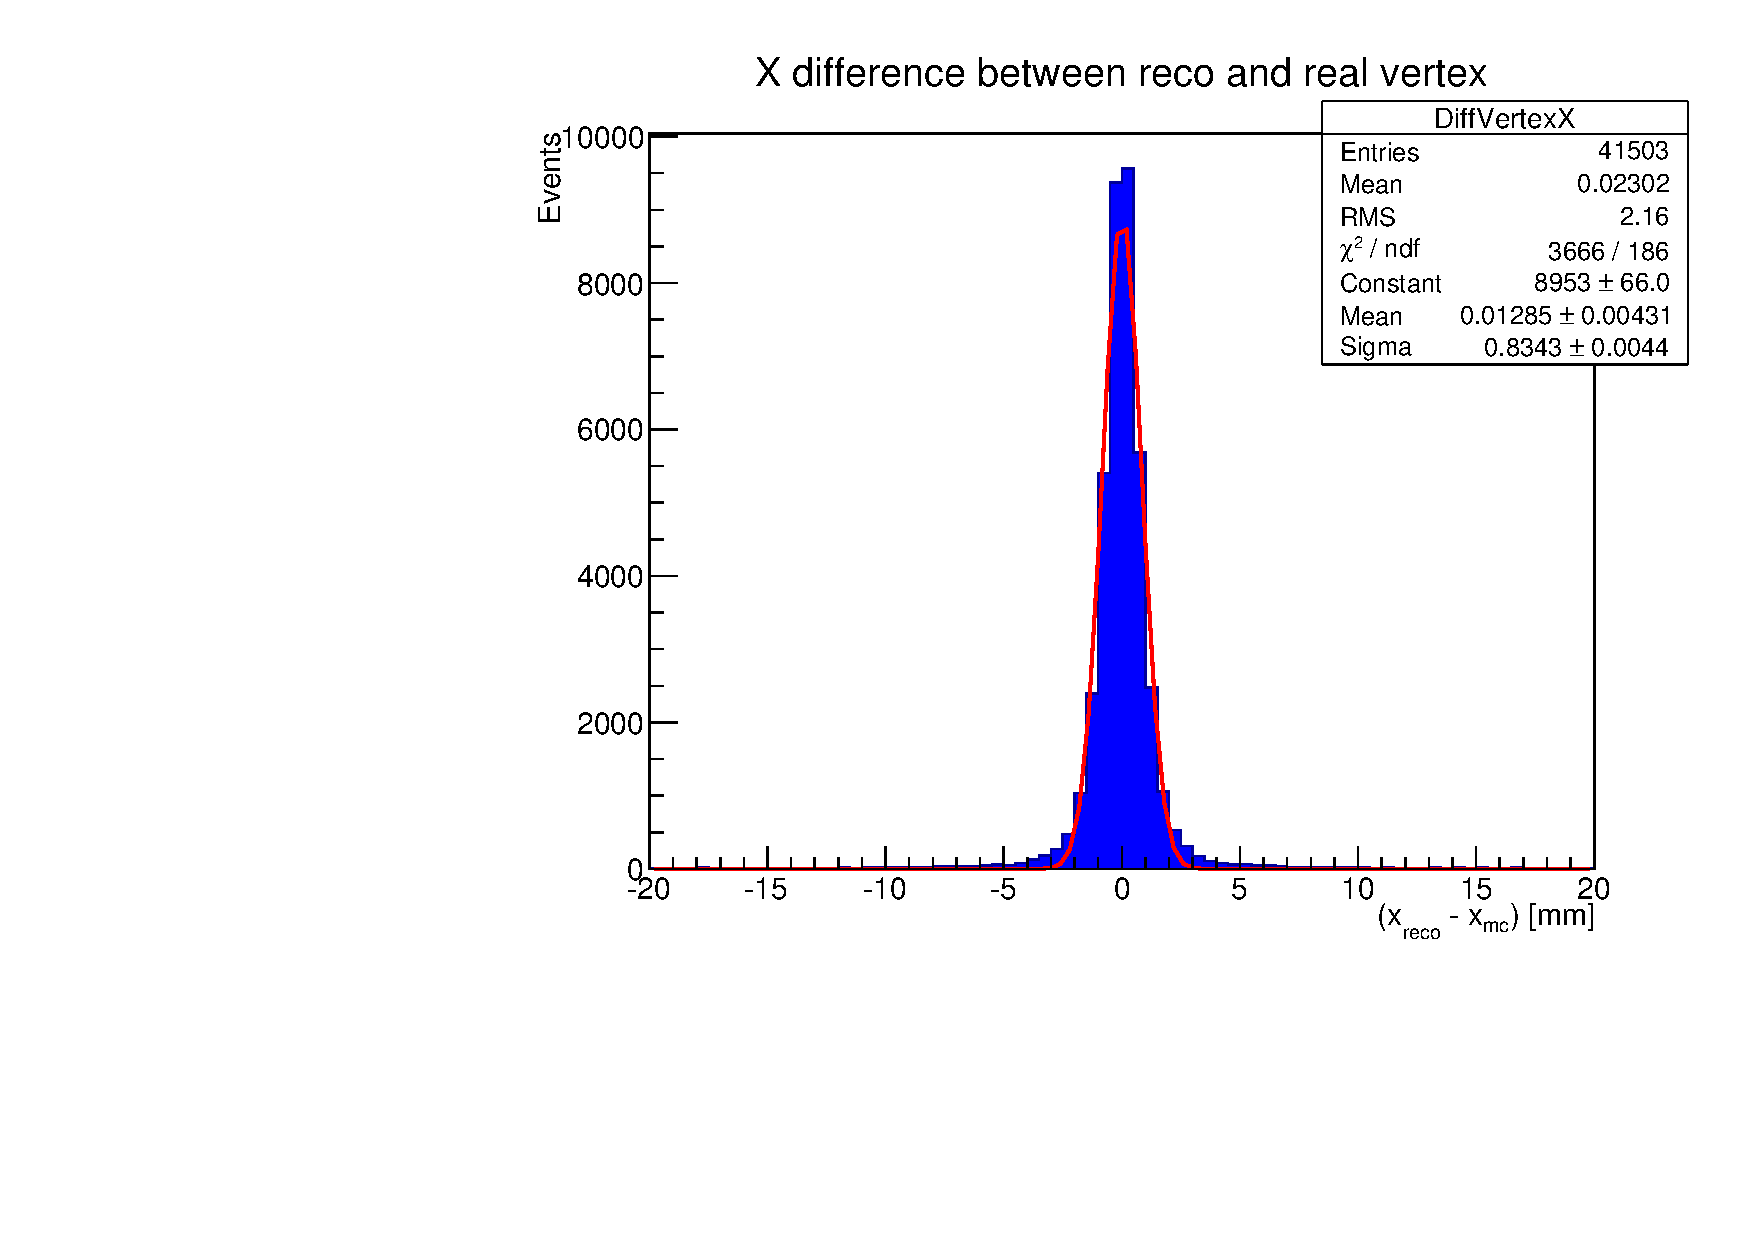
\includegraphics[width=\textwidth]{cdaxdiff}
\end{subfigure}
\begin{subfigure}{0.5\textwidth}
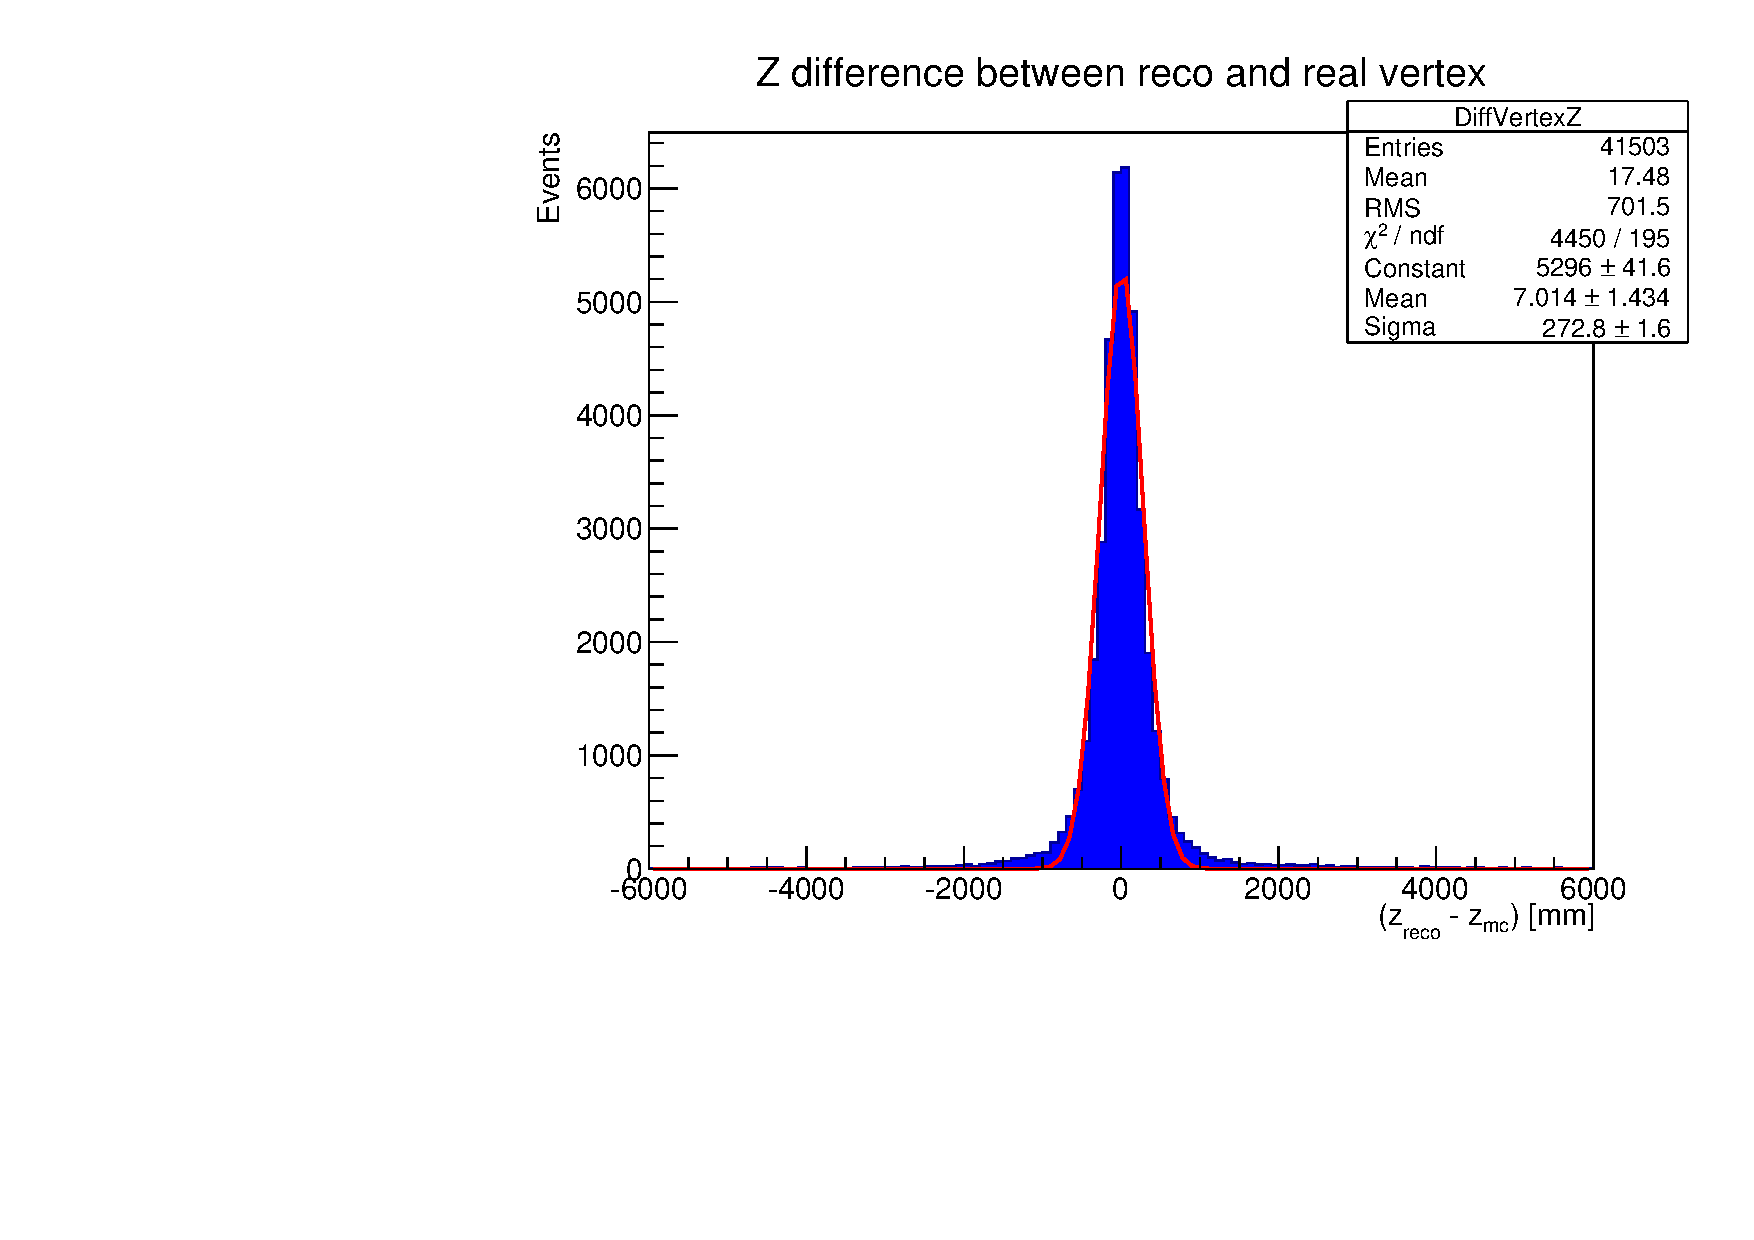
\includegraphics[width=\textwidth]{cdazdiff}
\end{subfigure}
\caption{Top: histograms of the reconstructed vertex x and z positions. Bottom: histograms of the
difference between the reconstructed and the real vertex x and z
positions}\label{vertexcdavalidation}
\end{figure}

